\documentclass[border=4pt]{standalone}
\usepackage{tikz}
\usetikzlibrary{arrows.meta,decorations.pathmorphing}
\definecolor{boxblue}{RGB}{225,238,252}
\definecolor{boxorange}{RGB}{253,236,216}
\definecolor{boxgray}{RGB}{237,237,237}
\begin{document}
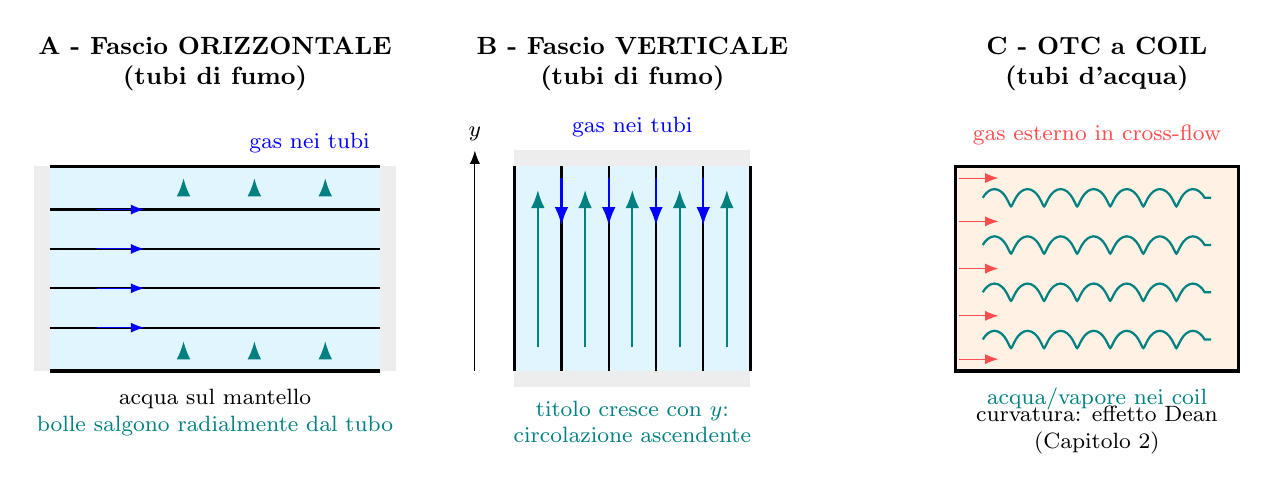
\begin{tikzpicture}[font=\footnotesize]

% ============ A: horizontal fire-tube ============
\begin{scope}[xshift=0cm, yshift=0cm]
\node[font=\small\bfseries,align=center] at (2.4,2.6) {A - Fascio ORIZZONTALE\\(tubi di fumo)};
\fill[cyan!12] (0.3,-1.3) rectangle (4.5,1.3);
\draw[very thick] (0.3,1.3) -- (4.5,1.3);
\draw[very thick] (0.3,-1.3) -- (4.5,-1.3);
\fill[boxgray] (0.1,-1.3) rectangle (0.3,1.3);
\fill[boxgray] (4.5,-1.3) rectangle (4.7,1.3);
\foreach \y in {-0.75,-0.25,0.25,0.75}{
  \draw[thick] (0.3,\y) -- (4.5,\y);
  \draw[-{Latex},blue] (0.9,\y) -- (1.5,\y);
}
\node[blue] at (3.6,1.6) {gas nei tubi};
\node at (2.4,-1.65) {acqua sul mantello};
\foreach \x in {2.0,2.9,3.8}{
  \draw[-{Latex},teal,thick] (\x,-1.15) -- (\x,-0.92);
  \draw[-{Latex},teal,thick] (\x,0.92) -- (\x,1.15);
}
\node[teal] at (2.4,-2.0) {bolle salgono radialmente dal tubo};
\end{scope}

% ============ B: vertical fire-tube ============
\begin{scope}[xshift=6.2cm, yshift=0cm]
\node[font=\small\bfseries,align=center] at (1.5,2.6) {B - Fascio VERTICALE\\(tubi di fumo)};
\fill[cyan!12] (0,-1.3) rectangle (3.0,1.3);
\draw[very thick] (0,-1.3) -- (0,1.3);
\draw[very thick] (3.0,-1.3) -- (3.0,1.3);
\fill[boxgray] (0,1.3) rectangle (3.0,1.5);
\fill[boxgray] (0,-1.5) rectangle (3.0,-1.3);
\foreach \x in {0.6,1.2,1.8,2.4}{
  \draw[thick] (\x,-1.3) -- (\x,1.3);
}
\foreach \x in {0.6,1.2,1.8,2.4}{\draw[-{Latex},blue,thick] (\x,1.15) -- (\x,0.55);}
\node[blue] at (1.5,1.8) {gas nei tubi};
\foreach \x in {0.3,0.9,1.5,2.1,2.7}{
  \draw[-{Latex},teal,thick] (\x,-1.0) -- (\x,1.0);
}
\node[teal,align=center] at (1.5,-1.95) {titolo cresce con $y$:\\ circolazione ascendente};
\draw[-{Latex}] (-0.5,-1.3) -- (-0.5,1.5) node[above]{$y$};
\end{scope}

% ============ C: OTC coil ============
\begin{scope}[xshift=11.8cm, yshift=0cm]
\node[font=\small\bfseries,align=center] at (1.8,2.6) {C - OTC a COIL\\(tubi d'acqua)};
\fill[orange!10] (0,-1.3) rectangle (3.6,1.3);
\draw[very thick] (0,-1.3) rectangle (3.6,1.3);
\foreach \y in {-0.9,-0.3,0.3,0.9}{
  \draw[thick,teal,decorate,decoration={coil,aspect=0.4,segment length=4.2mm,amplitude=1.1mm}] (0.35,\y) -- (3.25,\y);
}
\foreach \y in {-1.15,-0.6,0.0,0.6,1.15}{
  \draw[-{Latex},red!70] (0.05,\y) -- (0.55,\y);
}
\node[red!70] at (1.8,1.7) {gas esterno in cross-flow};
\node[teal] at (1.8,-1.65) {acqua/vapore nei coil};
\node[align=center] at (1.8,-2.05) {curvatura: effetto Dean\\(Capitolo 2)};
\end{scope}

\end{tikzpicture}
\end{document}
